\subsection{A first-round gain that does not persist under the same metric}
All four core acquisition/assessment phases pass the original strict raw
verifier. Each teacher evaluates 25,215 first-round acquisition geometries,
23,504 first-round assessment geometries, 40,301 second-round acquisition
geometries, and 27,725 second-round assessment geometries: 233,490
geometry--teacher evaluations in total. The first round adds exactly 2,304
new TRAIN rows per model/seed, shared across its three label policies.

\begin{table}[htbp]
\centering\small
\caption{Change in balanced H0 fixed-bin yield versus an equal-update no-new-data continuation, in percentage points, mean $\pm$ sample SD over three paired fit/proposal seeds. Round 2 uses the same first-round lineage as its control. The rounds have separate assessment histories.}
\begin{tabular}{lrrrr}\toprule
Model / rule & UMA r1 & UMA r2 & MACE r1 & MACE r2\\\midrule
AR / fixed & $-1.33\pm1.61$ & $+1.39\pm0.53$ & $-1.50\pm0.85$ & $+1.27\pm0.35$\\
AR / adaptive & $-0.35\pm1.51$ & $+0.61\pm0.60$ & $+0.03\pm2.23$ & $+0.14\pm0.90$\\
AR / range & $+6.57\pm2.36$ & $-5.41\pm1.48$ & $+6.13\pm1.35$ & $-6.31\pm1.65$\\
CVAE $D=2$ / fixed & $-0.90\pm0.88$ & $-0.17\pm0.68$ & $-0.69\pm1.00$ & $-0.55\pm0.56$\\
CVAE $D=2$ / adaptive & $+0.17\pm1.61$ & $+0.43\pm0.63$ & $+0.12\pm1.66$ & $+0.26\pm0.77$\\
CVAE $D=2$ / range & $+6.08\pm1.97$ & $-6.28\pm1.76$ & $+6.16\pm1.25$ & $-6.22\pm1.48$\\
\bottomrule\end{tabular}
\end{table}

\begin{table}[htbp]
\centering\small
\caption{Declared broad three-bin sampling baselines: balanced H0 yield in percent, mean $\pm$ three-seed SD. Mutation uses its frozen original-TRAIN seed bank. These numbers do not replace earlier LOW-only or differently seeded mutation studies.}
\begin{tabular}{llrr}\toprule
Round & Teacher & Uniform & Mutation\\\midrule
1 & UMA & $34.06\pm1.94$ & $58.36\pm0.53$\\
1 & MACE & $33.19\pm1.37$ & $57.18\pm0.41$\\
2 & UMA & $33.88\pm0.59$ & $58.16\pm1.53$\\
2 & MACE & $33.68\pm1.51$ & $56.63\pm1.18$\\
\bottomrule\end{tabular}
\end{table}


Observed-range labels give a clear first-round balanced-yield gain relative
to the declared no-new-data continuation. The same-data contrast is also
positive: range minus fixed gives $+7.90\pm0.83$ percentage points for AR
and $+6.97\pm2.74$ for $D=2$ under UMA; MACE gives $+7.64\pm0.76$ and
$+6.86\pm2.25$. These are three-fit sample SDs. This isolates the effect of
label definitions and induced class weighting on the same augmented rows,
rather than proving that acquisition itself was necessary.

The improvement is not uniform across requested classes. For AR, the
range-minus-fixed change is only $+0.35$ points for fixed-H0 LOW yield but
$+29.77$ points for HIGH yield. A balanced three-class gain should therefore
not be described as an equivalent gain in low-energy discovery. The
declared uniform and mutation baselines remain below the neural models in
this broad three-bin assessment. Different seed-selection or LOW-only
mutation studies have a different target and cannot be substituted here.

\begin{figure}[htbp]
\centering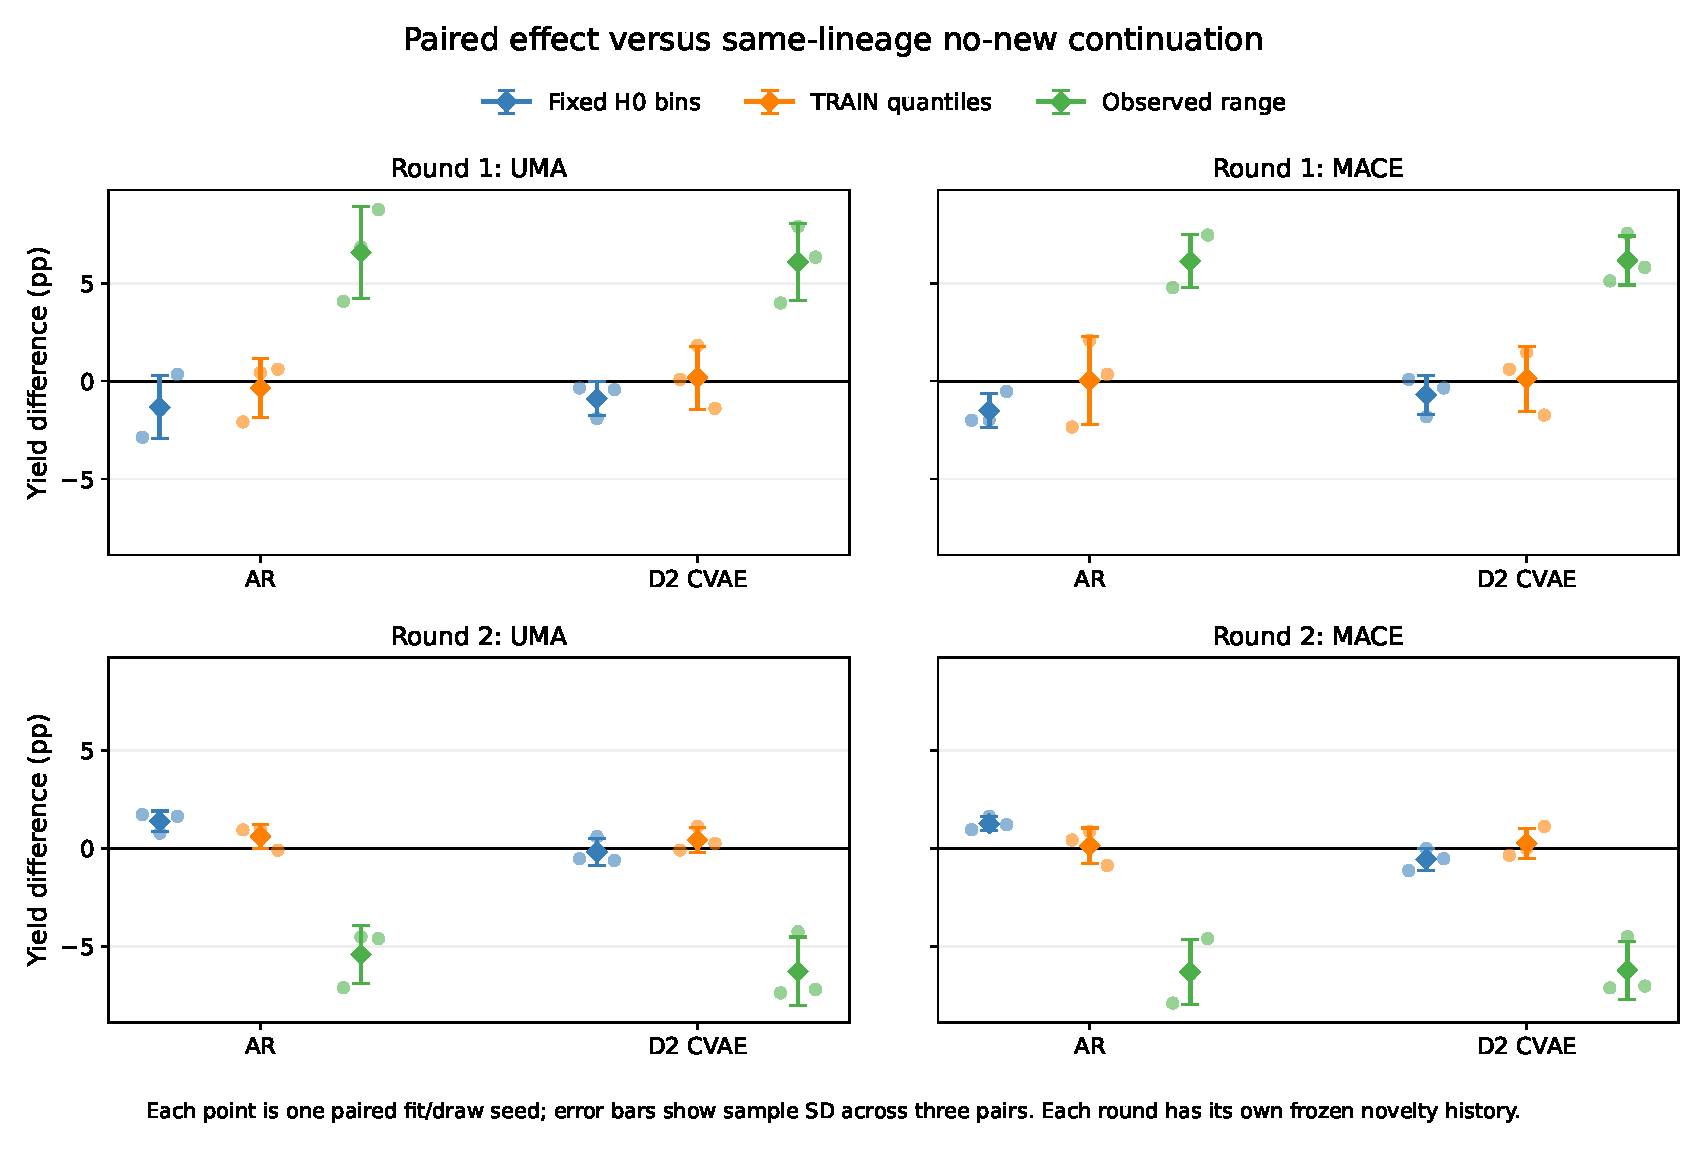
\includegraphics[width=\linewidth]{iteration_paired_gains.pdf}
\caption{Paired effects relative to the appropriate equal-update
continuation. Round 1 compares with H0 continuation; round 2 compares with
the same first-round lineage continued without a new batch. Individual
replicates and three-fit SD are shown. Fixed-H0 evaluation bins remain
constant; the novelty history is separately frozen for each round.}
\end{figure}

In round two, the range policy loses $5.41\pm1.48$ points for AR and
$6.28\pm1.76$ for $D=2$ relative to its same-lineage no-new-data control
under UMA. MACE gives corresponding losses of $6.31\pm1.65$ and
$6.22\pm1.48$ points. Absolute UMA range yields are 70.28\% and 68.66\%,
compared with the fresh uniform baseline 33.88\% and mutation 58.16\%.
Thus the neural sampler remains useful against these declared baselines,
while adding another range-policy batch does not sustain the first-round
improvement in the fixed-reference statistic.

\subsection{Novelty, condition fidelity, and the moving target}
Existing-result diagnostics separate novelty $N$ from conditional accuracy
$A$ among scored new orbits. Within each cell, $Y=NA$. The exact symmetric
rate decomposition is
\begin{equation}
\Delta Y=\tfrac12(A_1+A_0)\Delta N+
          \tfrac12(N_1+N_0)\Delta A.
\end{equation}
Balanced cell averages therefore retain an exact arithmetic decomposition;
it does not identify the causal training mechanism. For UMA range AR, the
round-two change is approximately $-1.06$ percentage points from the novelty
term and $-4.36$ from conditional accuracy. For $D=2$ the terms are
$-1.97$ and $-4.31$ points. Novelty remains 98.41\%/97.34\%, versus
99.51\%/99.33\% in the respective continuations. The dominant measured
change is condition fidelity, rather than wholesale repetition of known
patterns. Some LOW cells lose roughly 14 points despite almost complete
novelty.

There is an important target-alignment explanation to examine. For a
range-defined lower cutoff $a=0.8E_{\min}+0.2E_{\max}$,
$\Delta a=0.8\Delta E_{\min}+0.2\Delta E_{\max}$. The range acquisition
mostly extends the \emph{upper} energy endpoint, while its lower endpoint
changes much less. Raising $E_{\max}$ also raises the definition of LOW.
The generator can consequently match a broader, higher-energy LOW class
while losing hits under the original fixed-H0 LOW threshold. Moving-bin
fidelity and observed endpoint growth are therefore reported separately;
the fixed-yield loss alone does not establish failure to extend upper-energy
coverage. Nor does extending an observed range prove global coverage or
convergence.

\begin{figure}[htbp]
\centering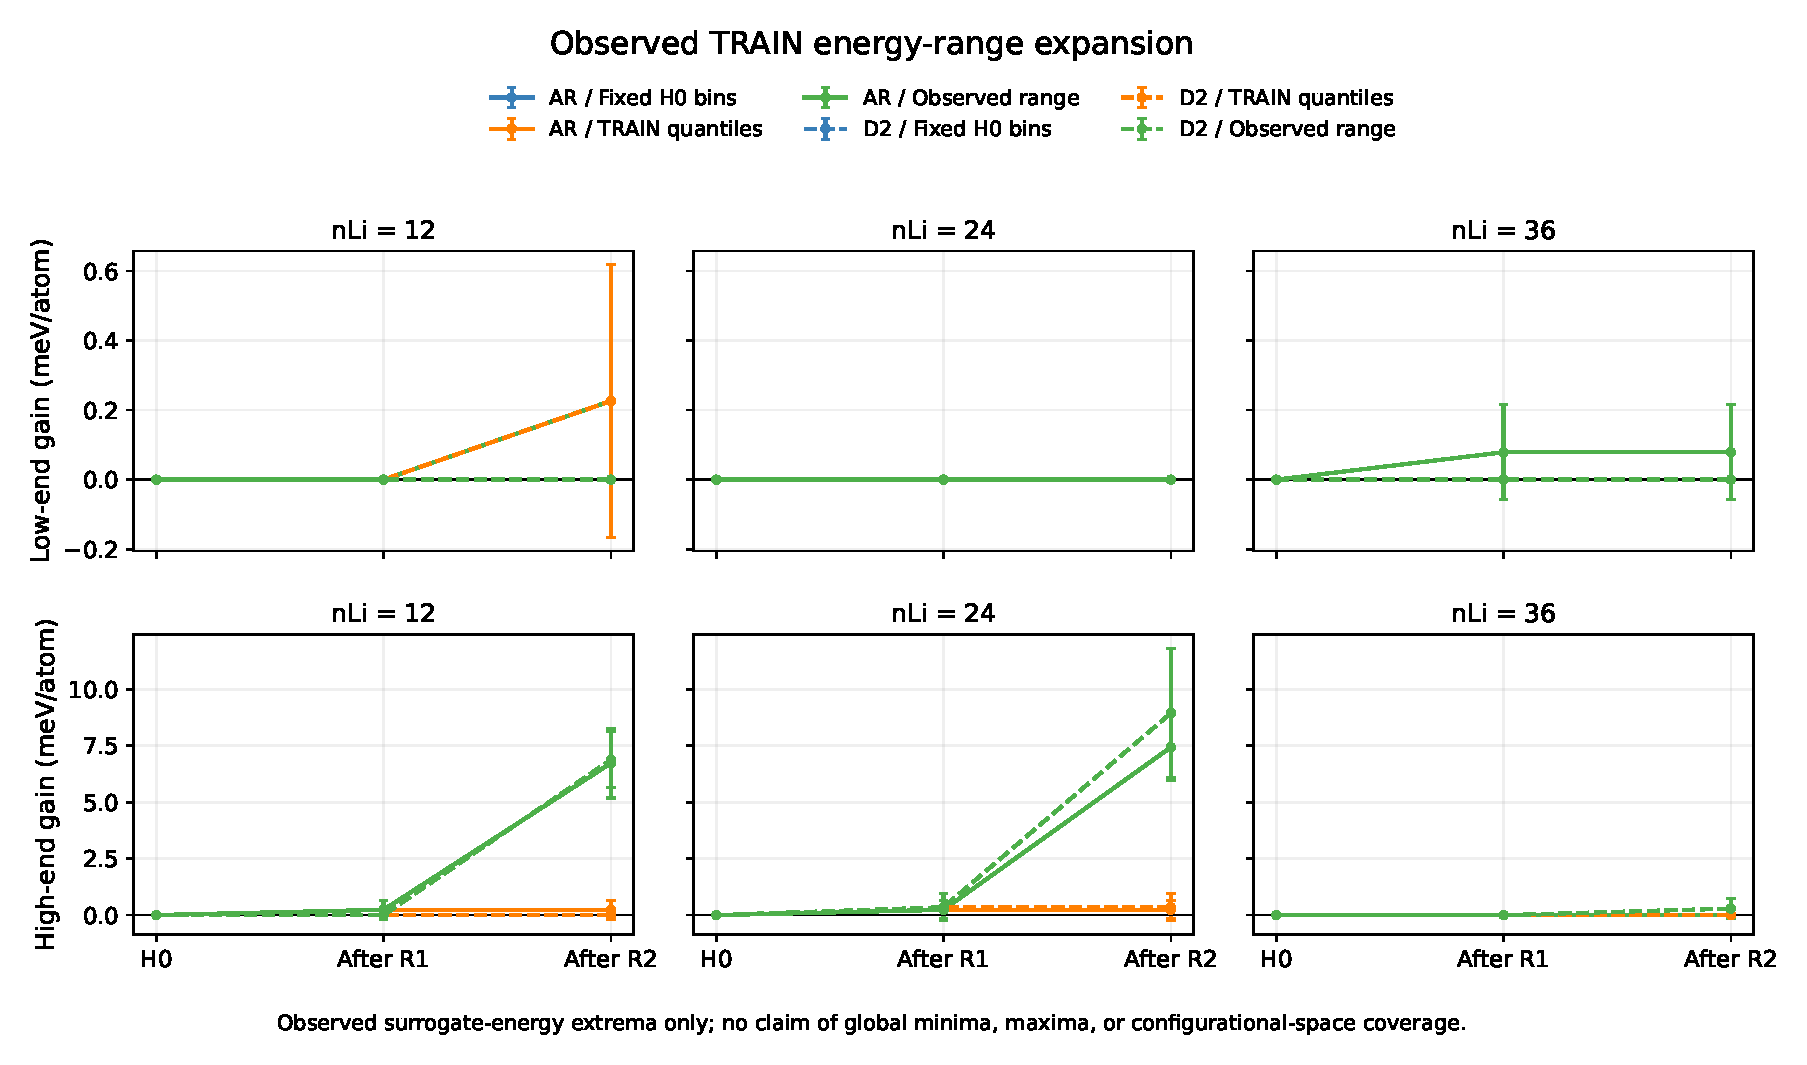
\includegraphics[width=\linewidth]{observed_training_extrema_growth.pdf}
\caption{Observed TRAIN endpoint extension relative to H0, within each
composition. Positive lower-endpoint growth means a lower observed minimum;
positive upper-endpoint growth means a higher maximum. These nested TRAIN
data can be compared longitudinally, unlike assessment yields with changing
novelty histories. Error bars are three-seed SD, not bounds on global extrema.}
\end{figure}

Range labels also concentrate the loss on rare examples. One first-round
36-Li HIGH class has only three TRAIN structures among roughly 14,000.
Class balancing changes per-row loss weights, not the uniformly shuffled
minibatch order. If those three examples carry one third of the within-count
loss mass, Cauchy's inequality gives $\sum_i p_i^2\geq1/27$ for normalized
weights $p_i$, hence weight ESS $1/\sum_i p_i^2\leq27$. This is concentration
of objective weight, not 27 independent physical observations. The first
round's positive result means sparsity alone cannot be cited as the cause
of the second-round loss. Actual class support, edge shifts, endpoint motion,
and weight ESS are all retained for each lineage.

\subsection{Does the first range-label gain require new structures?}
A post-hoc control separates two changes that occurred together in the first
round: adding newly evaluated structures and redefining their energy classes.
This follow-up was prompted by the first-round result; it is a mechanistic
test, not a new blind confirmation. Its plan and paired fit/proposal seeds were
frozen before the follow-up fits.

For each architecture and each of the three seeds, the comparison starts from
the same original 4,000-update checkpoint and allocates another 2,000 updates.
The original H0 data and first-round augmented data are each evaluated with
fixed bins and with identical range-bin edges. Existing equal-update
checkpoints supply the H0/fixed and augmented-data comparisons. We additionally
fit H0 with range edges estimated from H0 TRAIN alone, which tests relabeling
without any acquired labels. Some H0 and augmented-data range edges differ,
so six more H0 fits use each lineage's exact first-round range edges. These
remove edge location as a difference when testing the effect of added rows.
There are twelve new fits in total; all requested classes have actual H0
TRAIN support.

All compared checkpoints generate fresh proposals under one common history,
with 128 attempts for each count/request cell and common proposal streams.
Their energies are evaluated under the original, teacher-specific H0
assessment bins. None of these assessment labels enter training. The
comparison therefore asks whether new rows help under the same physical
energy intervals, rather than allowing the assessment target to move.

\begin{table}[htbp]
\centering\small
\caption{Posthoc conditioning/data controls: balanced H0 fixed-bin yield change, percentage points, mean $\pm$ sample SD over three paired fits. Relabeling also changes class-balanced loss weights. The matched-range comparison holds the physical edges identical; adding rows can still change minibatches and row weights.}
\begin{tabular}{lrr}\toprule
Model / contrast & UMA & MACE\\\midrule
AR / H0 range versus fixed & $+6.48\pm1.01$ & $+6.11\pm0.98$\\
AR / New rows / fixed edges & $-1.56\pm0.88$ & $-1.10\pm1.33$\\
AR / New rows / matched range edges & $-1.36\pm0.39$ & $-2.05\pm0.84$\\
CVAE $D=2$ / H0 range versus fixed & $+7.06\pm1.09$ & $+6.80\pm0.91$\\
CVAE $D=2$ / New rows / fixed edges & $+0.41\pm0.78$ & $+0.09\pm0.46$\\
CVAE $D=2$ / New rows / matched range edges & $+1.85\pm1.33$ & $+2.00\pm1.39$\\
\bottomrule\end{tabular}
\end{table}


Relabeling H0 alone recovers a large gain: $+6.48\pm1.01$ percentage points for
AR and $+7.06\pm1.09$ for $D=2$ under UMA. MACE gives
$+6.11\pm0.98$ and $+6.80\pm0.91$ points. The corresponding effect of adding
rows at identical first-round range edges is smaller and depends on the
architecture: $-1.36\pm0.39$ points for AR and $+1.85\pm1.33$ for $D=2$
under UMA, with MACE changes of $-2.05\pm0.84$ and $+2.00\pm1.39$.
Under the original fixed bins, adding rows changes UMA yield by
$-1.56\pm0.88$ for AR and $+0.41\pm0.78$ for $D=2$.
These are sample SDs over three paired fit/proposal replicates.

The large first-round gain can thus be obtained without acquiring new
structures. This supports a useful role for the definition of the conditioning
classes and the associated loss weighting. It does not establish that
acquisition is useless: added rows have a small positive effect for $D=2$
under matched range edges, and the acquisition pools extend the observed
upper-energy range. Nor does the control isolate why relabeling helps.
Relabeling changes class membership and the weights assigned by the
class-balanced loss; adding rows also changes minibatches and class weights.
The effects measured here belong to that declared training procedure.

\begin{figure}[htbp]
\centering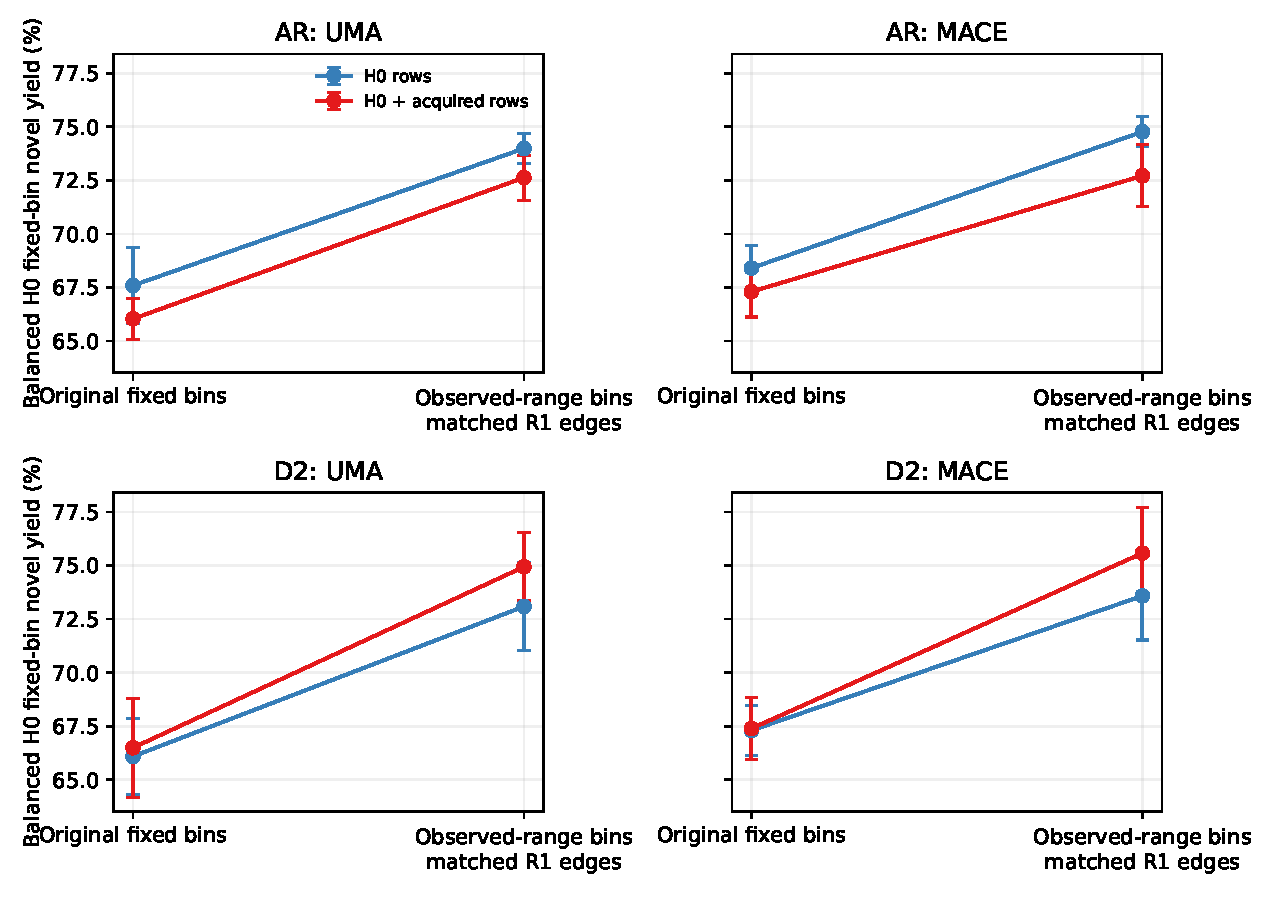
\includegraphics[width=\linewidth]{causal_factorial.pdf}
\caption{Post-hoc data-by-conditioning control on fresh common proposals.
The two data choices use identical physical condition edges at each plotted
position. The separate pure-H0 range fit, whose edges need no acquired labels,
is included in the control table. Error bars show three-pair sample SD.
The result concerns fixed-H0 conditional yield, not DFT accuracy or a
global energy minimum.}
\end{figure}

The follow-up completes in 18.04 minutes and uses 34,686 geometry--teacher
evaluations, with all raw-score checks passing. Its raw proposal identities
are reserved before the subsequent search pilot, preserving the assessment
boundary.

\subsection{A bounded test of explicit endpoint search}
Updating energy labels does not directly follow an energy gradient. We
therefore run a separate discrete search pilot to test the value of feedback
from an actual MLIP evaluation. It begins only after the core experiment is
complete and after all causal-control proposal identities have been reserved.

At each of the three lithium counts, LOW and HIGH searches begin from 16
unprotected H0 TRAIN masks per seed. Greedy and energy-blind walks share those
starts. At each of four steps, each trajectory proposes eight edits, each
exchanging one occupied and one vacant Li site. This is one swap in occupancy
space, not a physical diffusion trajectory. The greedy walk chooses the
lowest- or highest-energy eligible neighbor according to UMA; ties use a
declared canonical-mask order. The blind walk's chosen neighbor and its
eligibility-only fallback are written before any new energy is evaluated.
Both walks query the full eligible candidate union. Their first-step raw
proposals and query unions are checked to be exactly identical.

A uniform fixed-count sampler receives the same attempt/query caps, without
a claim of identical edit semantics. Each arm has at most 128 attempts and
new queries per count/direction/step, or 512 over four steps. Known,
protected, and repeated orbits remain excluded without top-ups. Actual
selected query counts are retained, and shared geometry--teacher evaluations
are physically performed only once.

\begin{table}[htbp]
\centering\small
\caption{Best observed UMA energy gain relative to the same starting-pool
best, in meV/atom, mean $\pm$ sample SD over three paired seeds. Positive
LOW gain means lower energy; positive HIGH gain means higher energy.
The reference is the best of the common 16 starts, not the minimum or
maximum of the entire H0 dataset.}
\begin{tabular}{llrrr}\toprule
Li count & Direction & Greedy & Blind walk & Uniform\\\midrule
12 & LOW  & $2.17\pm0.67$ & $1.38\pm0.97$ & $1.33\pm0.89$\\
24 & LOW  & $2.06\pm1.02$ & $1.05\pm0.65$ & $1.20\pm1.63$\\
36 & LOW  & $2.82\pm0.65$ & $1.21\pm0.29$ & $1.19\pm0.24$\\
12 & HIGH & $8.26\pm3.38$ & $3.70\pm0.14$ & $2.04\pm2.15$\\
24 & HIGH & $5.29\pm2.87$ & $4.61\pm3.34$ & $1.75\pm2.42$\\
36 & HIGH & $5.45\pm2.25$ & $1.93\pm1.31$ & $1.31\pm1.72$\\
\bottomrule\end{tabular}
\end{table}

Within this bounded budget, energy feedback improves the mean observed LOW
endpoint relative to both declared controls at all three counts. MACE audits
the same queried structures independently and shows the same qualitative
LOW advantage: greedy gains are 2.33, 2.16, and 2.46 meV/atom at counts
12, 24, and 36. MACE does not choose the next states. The HIGH advantage is
less uniform across counts and replicates, particularly at count 24.
These small paired experiments do not establish a universal ordering of
the methods.

\begin{figure}[htbp]
\centering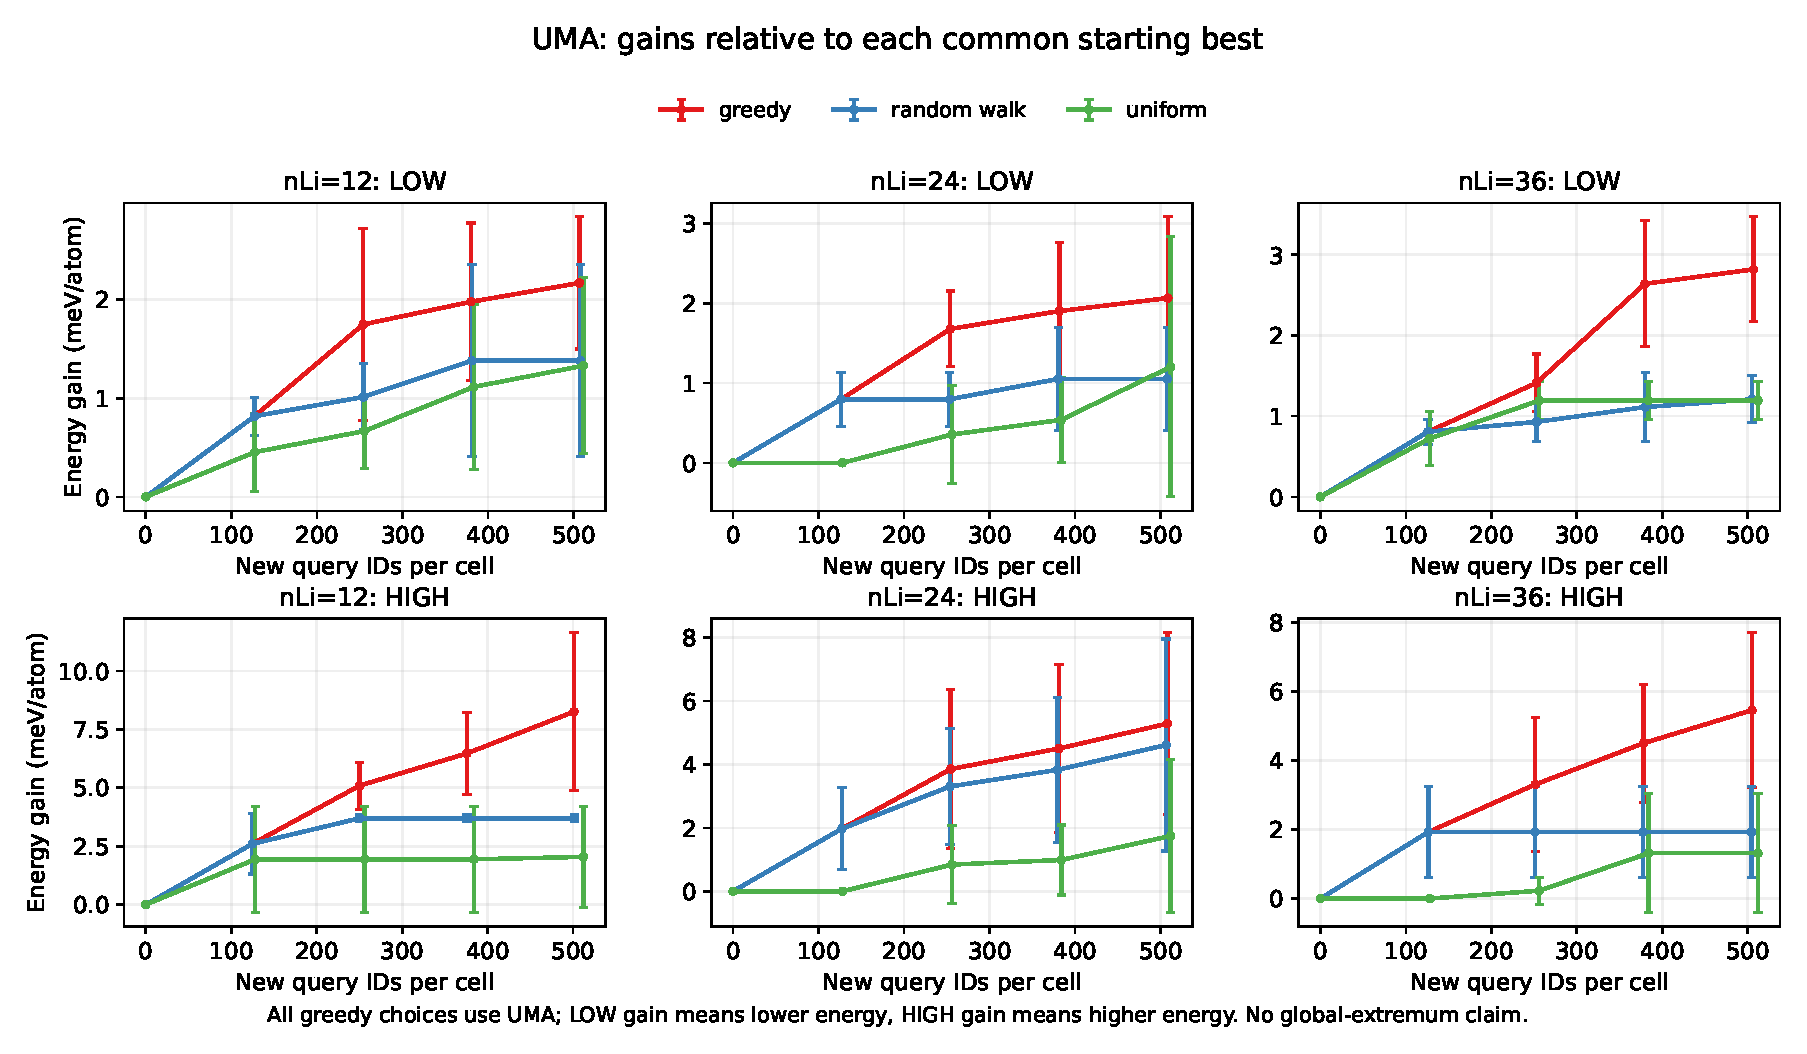
\includegraphics[width=\linewidth]{frontier_uma_best_gain.pdf}
\caption{Observed endpoint gains versus actual newly scored cell-query IDs.
Greedy and blind walks have identical first-step queries and fixed one-swap,
eight-neighbor budgets. Uniform has equal caps but different proposal
semantics. Best-so-far includes every evaluated neighbor and is monotone
by construction. Selected current paths are logged separately and may leave
an earlier best; the retained best and current state are different objects.
Error bars show three-seed sample SD.}
\end{figure}

No neural edit model is trained in this pilot. It separates label
redistribution from explicit oracle-guided search and cannot be treated as
a matched-edit comparison with the CVAE decoder. The new evaluations cover
49,570 geometry--teacher pairs, plus 574 separate rescoring evaluations of
287 distinct TRAIN seed masks. The pilot completes in 30.88 minutes within
its declared cap, with all raw checks passing.

Exact orbit filtering applies to all arms. Current-state uniqueness is
partly imposed by that filter, so it is not evidence of unrestricted
diversity. The saved diversity diagnostic instead uses the minimum Hamming
distance over parent symmetries, divided by two: the number of Li/vacancy
swaps separating two masks. The comparison uses the 16 current walk states
or the first 16 eligible uniform proposals without energy selection.
All coordinates remain unrelaxed. The results concern observed surrogate
endpoints, not global extrema, configurational entropy, equilibrium phase
stability, or DFT validation.

